\ifx\boi\undefined\ifx\problemname\undefined
\providecommand\sampleinputname{}
\providecommand\sampleoutputname{}
\documentclass[norsk]{templates/boi}
\problemlanguage{.no}
\fi
\newcommand{\boi}{Baltic Olympiad in Informatics}
\newcommand{\practicesession}{Practice Session}
\newcommand{\contestdates}{April 27 - May 1, 2018}
\newcommand{\dayone}{Dag 1}
\newcommand{\daytwo}{Dag 2}
\newcommand{\licensingtext}{This problem is licensed under CC BY-SA 4.0.}
\newcommand{\problem}{Problem}
\newcommand{\inputsection}{Input}
\newcommand{\outputsection}{Output}
\newcommand{\interactivity}{Interaktivitet}
\newcommand{\grading}{Grading}
\newcommand{\scoring}{Scoring}
\newcommand{\constraints}{Begrensninger}
\renewcommand{\sampleinputname}{Sample Input}
\renewcommand{\sampleoutputname}{Sample Output}
\newcommand{\sampleexplanation}[1]{Forklaring av eksempel #1}
\newcommand{\sampleexplanations}{Eksempelforklaring}
\newcommand{\timelimit}{Time Limit}
\newcommand{\memorylimit}{Memory Limit}
\newcommand{\seconds}{s}
\newcommand{\megabytes}{MB}
\newcommand{\group}{Group}
\newcommand{\points}{Points}
\newcommand{\limitsname}{Limits}
\newcommand{\additionalconstraints}{Yttligere begrensninger}
\newcommand{\testgroups}{
Løsningen din vil bli testet på et sett av testgrupper, hver verdt et visst antall poeng.
Hver testgruppe inneholder et sett av tester.
For å få poeng for en testgruppe må du løse alle testene i den gruppen.
Din endelige poengsum vil være den høyeste poengsummen du har fått på en enkelt innlevering.
}
\fi
\def\version{jury-1}
\problemname{Paths}
En {\em graf} er en matematisk struktur som består av et sett av {\em noder}, og et sett av {\em kanter}, hvor hver kant forbinder to noder. Et eksempel på en graf med $4$ noder og $3$ kanter er vist i eksempelforklaringen under.

En {\em sti} i en graf er definert som en ordnet liste av $2$ eller flere noder, slik at det finnes kanter mellom
hvert par av påfølgende noder i listen. I denne oppgaven er vi bare interresert i {\em enkle stier}
som er de hvor ingen noder opptrer mer enn én gang. Merk at listen er ordnet, så for eksempel representerer
``\texttt{5-6-7}'', ``\texttt{5-7-6}'' og ``\texttt{7-6-5}'' alle forskjellige stier.

%For example, a road map could be a graph, if the vertices are towns or other places and the edges are roads that directly connect two places.

I denne oppgaven er hver node i grafen fargelagt med en av $K$ forskjellige farger. Oppgaven går ut på å finne antall
(enkle) stier hvor alle nodene har forskjellige farger.

\section*{\inputsection}
Første linje i input inneholder tre heltall: $N$ (antall noder), $M$ (antall kanter), og $K$ (antall forskjellige farger).

%($1 \le N, M \le 3 \cdot 10^5, 1 \le K \le 5$).

Andre linje av input inneholder $N$ heltall mellom $1$ og $K$ -- fargene på hver av node i grafen (begynnende med node $1$ og sluttende med $N$).

Hver av de neste $M$ linjene beskriver en kant og inneholder to heltall $a, b$ ($1 \le a, b \le N, a \neq b$)
-- de to nodene som er forbundet med kanten. Det vil være maksimalt én kant mellom ett par av noder.

\section*{\outputsection}
Skriv ut ett heltall -- antall stier hvor alle nodene har forskjellige farger. Dette tallet vil alltid være mindre enn $10^{18}$.

\section*{\constraints}
\testgroups

\noindent
\begin{tabular}{| l | l | l |}
\hline
\group & \points & \limitsname \\ \hline
1      & 23      & $1 \le N, M \le 100, 1 \le K \le 4$ \\ \hline
2      & 20      & $1 \le N, M \le 300\,000, 1 \le K \le 3$ \\ \hline
3      & 27      & $1 \le N, M \le 300\,000, 1 \le K \le 4$ \\ \hline
4      & 30      & $1 \le N, M \le 100\,000, 1 \le K \le 5$ \\ \hline
\end{tabular}

\section*{\sampleexplanation{1}}

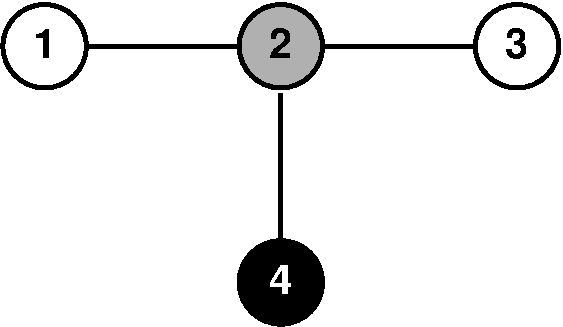
\includegraphics[width=5cm]{pathsfig.pdf}

Grafen i det første eksempelet er vist i figuren, hvor hvert punkt er fylt i enten hvitt (farge 1), grå (farge 2) eller svart (farge 3).
Det er 10 stier hvor alle nodene har forskjellige farger: ``\texttt{1-2}'', ``\texttt{2-1}'', ``\texttt{2-3}'', ``\texttt{3-2}'', ``\texttt{2-4}'', ``\texttt{4-2}'', ``\texttt{1-2-4}'', ``\texttt{4-2-1}'', ``\texttt{3-2-4}'' og ``\texttt{4-2-3}''.

Merk at ``\texttt{1}'' ikke er godkjent som en sti, fordi den består av bare én node. Ei heller er ``\texttt{1-2-3}'' lov, fordi den inneholder to noder med farge $1$.
